% ============================================================================
% Scalar QED: electron-muon scattering at lowest order (Pascal-triangle cell (1,1), n = 2)
%        phi_e(p) + phi_mu(k)  ->  phi_e(p') + phi_mu(k')       (two different charged scalars)
%
%   scalar "electron" = blue (top line)   scalar "muon" = red (bottom line)   photon = black wavy line
%   scalar lines are dashed (arrow = direction of charge flow); external scalars carry no spinor (factor 1).
%
% Conventions (Peskin & Schroeder, D_mu = d_mu + i e A_mu):
%   scalar-scalar-photon vertex   -i e (p + p')^mu     (p, p' = momenta along the charge arrow)
%   photon propagator             -i g_{mu nu}/(q^2 + i eps)   (Feynman gauge)
% Page = PowerPoint widescreen (13.333in x 7.5in).  Compile with pdflatex or lualatex.
% ============================================================================
\documentclass[10pt]{article}
\usepackage{lmodern}
\usepackage[T1]{fontenc}
\usepackage{amsmath,amssymb}
\usepackage{xcolor}
\usepackage{graphicx}
\usepackage{tikz}
\usetikzlibrary{decorations.markings,decorations.pathmorphing,arrows.meta,positioning}
\usepackage[paperwidth=338.67mm,paperheight=190.5mm,
            left=5mm,right=5mm,top=3mm,bottom=3mm]{geometry}
\pagestyle{empty}
\setlength{\parindent}{0pt}

\definecolor{ecol}{HTML}{1F4E9C}   % electron
\definecolor{mcol}{HTML}{C0392B}   % muon

\tikzset{
  bs/.style={line width=2.4pt,dash pattern=on 9pt off 5.5pt},  % scalar line (dashed)
  bar/.style={decoration={markings,                          % charge-flow arrow (solid tip), colour = argument
      mark=at position 0.55 with {\arrow{Stealth[length=5.6mm,width=4.8mm,color=#1,line width=2.4pt]}}},
    decorate},
  bph/.style={line width=1.8pt,decorate,                     % photon
    decoration={snake,amplitude=2.4pt,segment length=10.5pt}},
  bmom/.style={-{Stealth[length=2.8mm,width=2.3mm]},line width=1pt,color=black!70},
  elab/.style={font=\fontsize{30}{34}\selectfont,text=ecol,inner sep=2pt},
  mlab/.style={font=\fontsize{30}{34}\selectfont,text=mcol,inner sep=2pt},
  plab/.style={font=\fontsize{28}{32}\selectfont,inner sep=2pt},
  evbox/.style={font=\fontsize{30}{34}\selectfont,text=ecol,draw=ecol,fill=ecol!8,
                line width=1.2pt,rounded corners=4pt,inner sep=7pt},
  mvbox/.style={font=\fontsize{30}{34}\selectfont,text=mcol,draw=mcol,fill=mcol!8,
                line width=1.2pt,rounded corners=4pt,inner sep=7pt},
  pbox/.style={font=\fontsize{30}{34}\selectfont,draw=black!60,fill=black!4,
               line width=1.2pt,rounded corners=4pt,inner sep=8pt},
}

\begin{document}
\vspace*{\fill}
\centering
\scalebox{1.22}{%
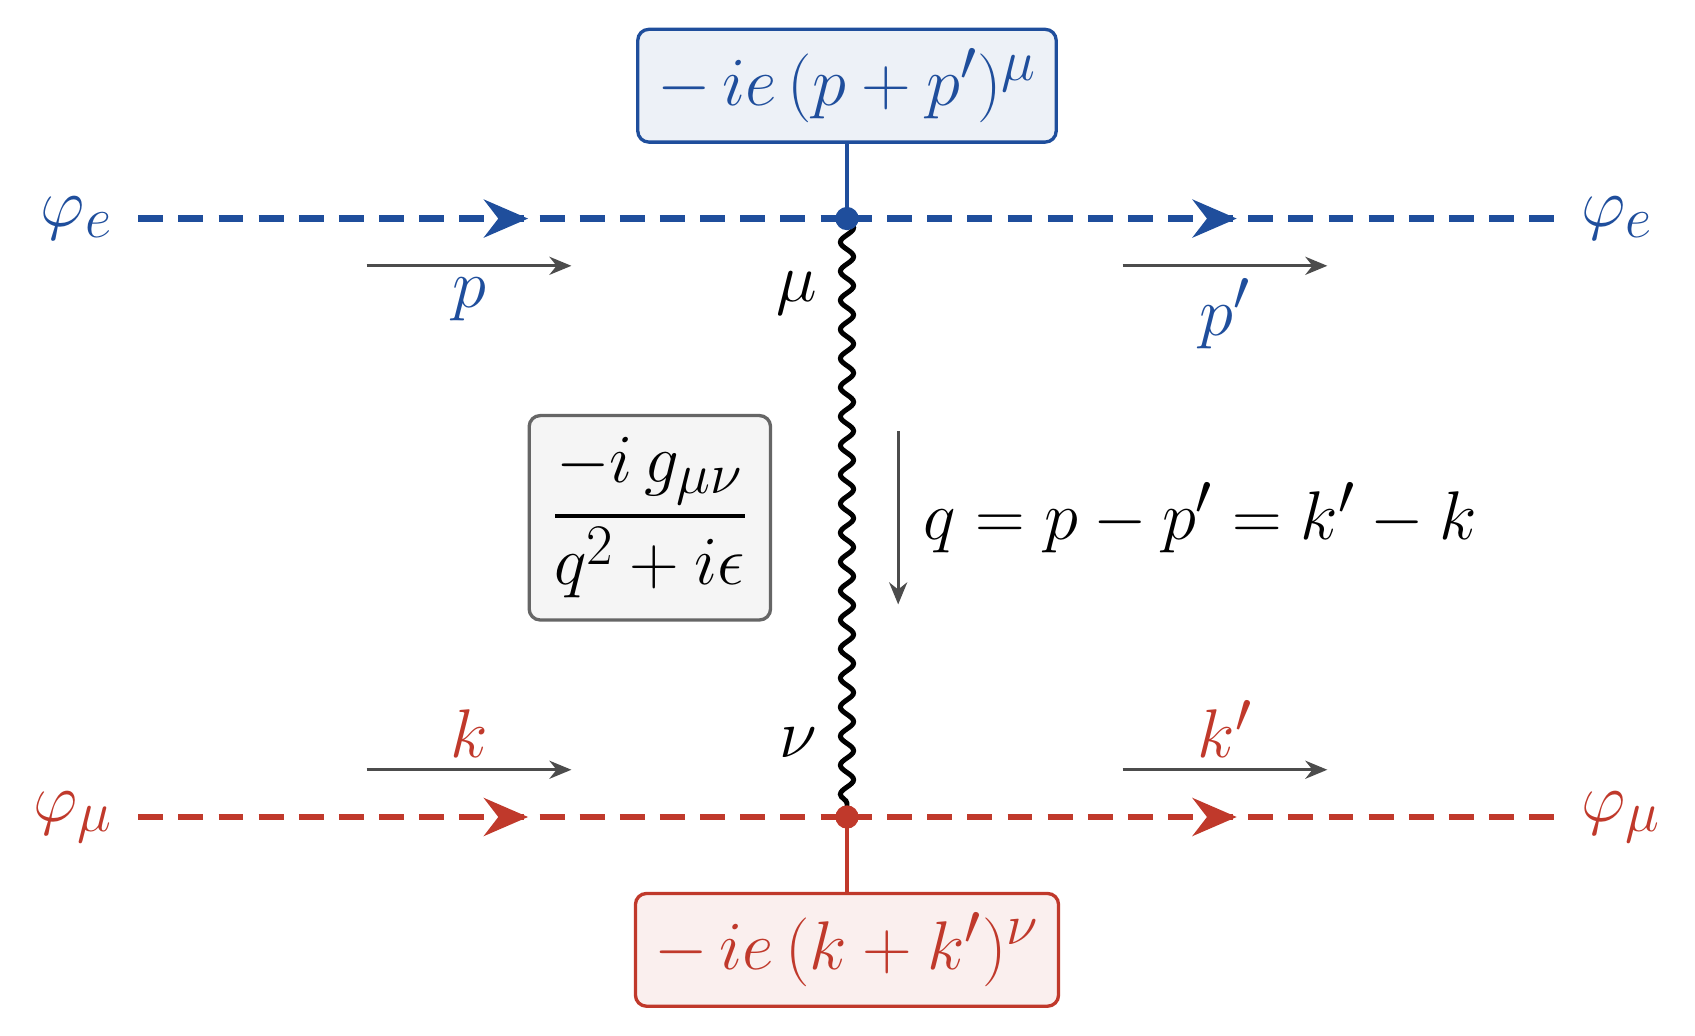
\begin{tikzpicture}[x=1cm,y=1cm]
  % ----------------------------------------------------------- scalar lines
  \draw[bs,color=ecol] (-9,3.8) -- (0,3.8);            % incoming scalar electron
  \draw[bs,color=ecol] ( 0,3.8) -- (9,3.8);            % outgoing scalar electron
  \draw[bs,color=mcol] (-9,-3.8) -- (0,-3.8);          % incoming scalar muon
  \draw[bs,color=mcol] ( 0,-3.8) -- (9,-3.8);          % outgoing scalar muon
  \path[bar=ecol] (-9,3.8)  -- (0,3.8);   \path[bar=ecol] (0,3.8)  -- (9,3.8);
  \path[bar=mcol] (-9,-3.8) -- (0,-3.8);  \path[bar=mcol] (0,-3.8) -- (9,-3.8);

  % ----------------------------------------------------------- photon
  \draw[bph] (0,3.8) -- (0,-3.8);

  % ----------------------------------------------------------- vertices (dots + boxed vertex factors)
  \fill[ecol] (0,3.8)  circle (4.2pt);
  \fill[mcol] (0,-3.8) circle (4.2pt);
  \draw[ecol,line width=1.2pt] (0,3.8)  -- (0,4.75);
  \draw[mcol,line width=1.2pt] (0,-3.8) -- (0,-4.75);
  \node[evbox,anchor=south] at (0,4.75)  {$-\,i e\,(p+p')^{\mu}$};
  \node[mvbox,anchor=north] at (0,-4.75) {$-\,i e\,(k+k')^{\nu}$};

  % ----------------------------------------------------------- particle names at the line ends
  \node[elab,anchor=east] at (-9.25,3.8)  {$\varphi_e$};
  \node[elab,anchor=west] at ( 9.25,3.8)  {$\varphi_e$};
  \node[mlab,anchor=east] at (-9.25,-3.8) {$\varphi_\mu$};
  \node[mlab,anchor=west] at ( 9.25,-3.8) {$\varphi_\mu$};

  % ----------------------------------------------------------- momenta (inside, between the lines)
  \draw[bmom] (-6.1,3.2) -- (-3.5,3.2);  \node[plab,anchor=north,text=ecol] at (-4.8,3.12) {$p$};
  \draw[bmom] ( 3.5,3.2) -- ( 6.1,3.2);  \node[plab,anchor=north,text=ecol] at ( 4.8,3.12) {$p'$};
  \draw[bmom] (-6.1,-3.2) -- (-3.5,-3.2); \node[plab,anchor=south,text=mcol] at (-4.8,-3.12) {$k$};
  \draw[bmom] ( 3.5,-3.2) -- ( 6.1,-3.2); \node[plab,anchor=south,text=mcol] at ( 4.8,-3.12) {$k'$};

  % ----------------------------------------------------------- photon: indices, momentum, propagator
  \node[plab,anchor=east] at (-0.3, 2.85)  {$\mu$};
  \node[plab,anchor=east] at (-0.3,-2.85)  {$\nu$};
  \draw[bmom] (0.65,1.1) -- (0.65,-1.1);
  \node[plab,anchor=west] at (0.9,0) {$q=p-p'=k'-k$};
  \node[pbox,anchor=east] at (-0.95,0) {$\displaystyle\frac{-i\,g_{\mu\nu}}{q^{2}+i\epsilon}$};
\end{tikzpicture}}
\vfill
\end{document}
